% ------------------ MALER ------------------
\begin{comment}

	\begin{question}[name=Oppgave, topic=forsterkning]

		\begin{enumerate}[label=\roman*)]

		\end{enumerate}
	\end{question}

	\vspace{0.5cm} % Add space after the solution

	\begin{solution}[name=Løsningsforslag oppgave]

		\begin{figure}[H]
			\centering
			\includegraphics[width=0.7\textwidth]{}
			\caption{}
			\label{fig:}
		\end{figure}
	\end{solution}
\end{comment}


\begin{question}[name=Oppgave, topic=forsterkning]
Beregn den totale forsterkningen av kretsen vist i Figur \ref{fig:forsterk1}.
	\begin{enumerate}[label=\roman*)]
	\item Beregn den totale forsterkningen ved å benytte $gain$
	\item Beregn den totale forsterkningen ved å benytte $gain_{dB}$ og diskuter resultatet.
	\end{enumerate}

	\begin{figure}[H]
	\centering
	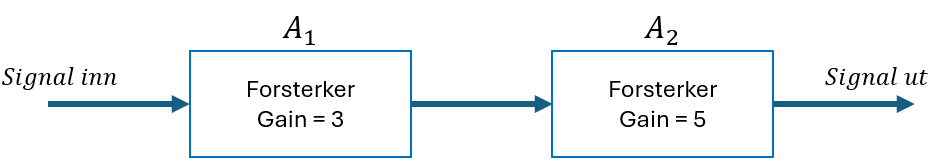
\includegraphics[width=0.9\textwidth]{forsterkning/figurer/forsterkning1.png}
	\caption{Forsterkning av signal}
	\label{fig:forsterk1}
\end{figure}
\end{question}

\vspace{0.5cm} % Add space after the solution

\begin{solution}[name=Løsningsforslag oppgave]
	\begin{enumerate}[label=\roman*)]
		\item Den totale forsterkningen kan man finne ved å multiplisere verdiene for $Gain$.

\[F_{tot}=F_{A1} \cdot F_{A2}= 3 \cdot 5 = 15\]

Konverterer til $dB$.
\[L_F=10 \cdot F_{tot} = 10 \cdot \log 15 = 11,76[dB]\]

	\item Finner nå totale forsterkningen i $[dB]$ ved å konvertere delverdiene og til slutt summere de samme for å få kretsens totale forsterkning.

\[L_{FA1}=10\cdot \log F_{A1} \rightarrow L_{FA1}=10 \cdot \log 3 \approx 4,77 [dB]\]
\[L_{FA2}=10 \cdot \log F_{A2} \rightarrow L_{FA2}=10 \cdot \log 5 \approx 6,99 [dB]\]
\[L_F = L_{FA1}+L_{FA2} = 4,77+6,99 = 11,76 [dB]\]

Basert på beregningen kan man observere at resultatet blir det samme for begge metoder.

	\end{enumerate}

\end{solution}
\vspace{0.5cm} % Add space after the solution


\begin{question}[name=Oppgave, topic=forsterkning]
Effekten inn i en forsterker er oppgitt til $1[W]$ når effekten ut er $10[W]$. Beregn forsterkningen i $[dB]$.
\end{question}

\vspace{0.5cm} % Add space after the solution

\begin{solution}[name=Løsningsforslag oppgave]
\[L_{FP}=10\cdot \log \frac{P_{ut}}{P_{inn}} \rightarrow L_{FP}=10 \cdot \log\frac{10}{1}=10[dB]\]

\end{solution}


\vspace{0.5cm} % Add space after the solution

\begin{question}[name=Oppgave, topic=forsterkning]
Beregn effektforsterkningen $F$ ved en forsterkning på $L_{FP}=20[dB]$
\end{question}

\vspace{0.5cm} % Add space after the solution

\begin{solution}[name=Løsningsforslag oppgave]
\[L_{FP}=10 \cdot \log F \rightarrow \]
Setter inn tall
\[20=10 \cdot \log F \rightarrow \frac{20}{10}= \log F\]

Tar så inverse funksjon av $ \log $ som er å oppheve begge sider med $10$.

\[10^2=10^{\log F} \rightarrow F=100\]

\end{solution}


\vspace{0.5cm} % Add space after the solution

\begin{question}[name=Oppgave, topic=forsterkning]
Spenningen inn i en forsterker er $10[mV]$ og spenningen over en $600[\Omega]$ last er $1[V]$. Beregn forsterkningen i $[dB]$.
\end{question}

\vspace{0.5cm} % Add space after the solution

\begin{solution}[name=Løsningsforslag oppgave]
Tegner opp en skisse av beskrivelsen som vist i \ref{fig:forsterk2}.
	\begin{figure}[H]
		\centering
		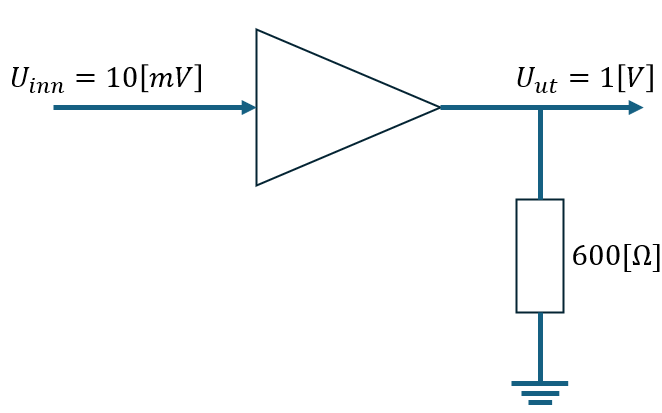
\includegraphics[width=0.5\textwidth]{forsterkning/figurer/forsterkningxLOS.png}
		\caption{Skisse for forsterkning av signal}
		\label{fig:forsterk2}
	\end{figure}

	Beregner spenningforsterkningen.
\[L_{FU} = 20 \cdot \log \frac{U_{ut}}{U_{inn}} \rightarrow L_{FU}=20 \cdot \log \frac{1}{10 \cdot 10 ^{-3}}= 40 [dB]\]

\end{solution}


\vspace{0.5cm} % Add space after the solution


\begin{question}[name=Oppgave, topic=forsterkning]
Hva er spenningen ut til instrumentet som vist i \ref{fig:forsterk3} dersom signalet fra sensoren er $2[mV]$?

	\begin{figure}[H]
	\centering
	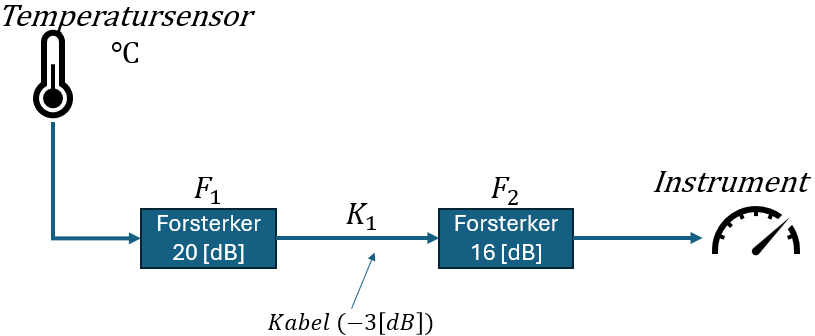
\includegraphics[width=0.7\textwidth]{forsterkning/figurer/forsterkning2.png}
	\caption{Forsterkning i et system}
	\label{fig:forsterk3}
\end{figure}
\end{question}

\vspace{0.5cm} % Add space after the solution

\begin{solution}[name=Løsningsforslag oppgave]
Summerer kretsens tre elementer. To elementer forsterker signalet, også en kabel som demper signalet. Dette kan man identifisere ved å se på fortegn.

Finner systemets totale forsterkning.
\[L_{FU_{tot}}=L_{F1}+L_{F2}+L_{F3}=20+(-3)+16= 33 [dB]\]

Konverterer tallet til enhetsløs forsterkning $F$.
\[L_{FU_{tot}} = 20 \cdot \log \frac{U_{ut}}{U_{inn}} \rightarrow 33=20 \cdot \log \frac{u_{ut}}{2 \cdot 10^{-3}} \rightarrow \frac{33}{20}=\frac{20}{20} \cdot \log \frac{U_{ut}}{2 \cdot 10`{-3}} \rightarrow 1,65 = \log \frac{u_{ut}}{2 \cdot 10^{-3}}\]

Tar invers av $log$.
\[10^{1,65} = 10^{log \frac{U_{ut}}{2 \cdot 10^{-3}}} \rightarrow 44,67 = \frac{U_{ut}}{2 \cdot 10^{-3}} \rightarrow U_{ut}=89,3[mV]\]
\end{solution}

\vspace{0.5cm} % Add space after the solution

\begin{question}[name=Oppgave, topic=forsterkning]
Hva er spenningen ut fra kretsen vist i \ref{fig:forsterk4}?

	\begin{figure}[H]
		\centering
		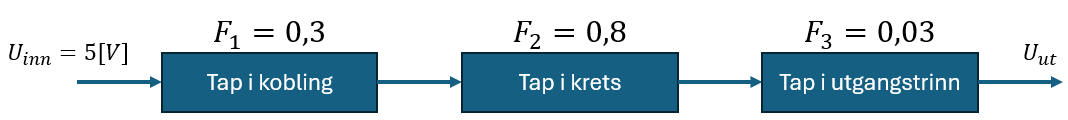
\includegraphics[width=0.9\textwidth]{forsterkning/figurer/forsterkning3.png}
		\caption{Forsterkning i et system}
		\label{fig:forsterk4}
	\end{figure}
\end{question}

\vspace{0.5cm} % Add space after the solution

\begin{solution}[name=Løsningsforslag oppgave]
Finner den totale dempingen.
\[F_{tot}= F_1 \cdot F_2 \cdot F_3 = 0,3 \cdot 0,8 \cdot 0,03 = 7,2 \cdot 10^{-3}\]

\[F_{tot}=\frac{U_{ut}}{U_{inn}} \rightarrow U_{ut}=f_{tot} \cdot U_{inn}=7,2 \cdot 10^{-3} \cdot 5 = 36[mV]\]

\end{solution}


\vspace{0.5cm} % Add space after the solution


\begin{question}[name=Oppgave, topic=forsterkning]
En effektforsterker har oppgitt en forsterkning på $40 [dB]$ med en effekt ut på $100[W]$. Hva er effekten inn i forsterkeren ved disse forholdene?
\end{question}

\vspace{0.5cm} % Add space after the solution

\begin{solution}[name=Løsningsforslag oppgave]
\[L_{FP}=10 \cdot \log \frac{p_{ut}}{P_{inn}} \rightarrow \frac{L_{FP}}{10}=\log \frac{P_{ut}}{P_{inn}}\]

Tar invers av $\log$.
\[10^{\frac{L_{FP}}{ 10}}= 10^{\log \frac{P_{ut}}{P_{inn}}} \rightarrow 10^{\frac{40}{10}}=10^{\log \frac{100}{P_{inn}}} \rightarrow 10000= \frac{100}{P_{inn}} \rightarrow P_{inn}=\frac{100}{10000}=10[mW]\]

\end{solution}


\vspace{0.5cm} % Add space after the solution




\begin{question}[name=Oppgave, topic=forsterkning]
Et signalanlegg er koblet opp som vist i Figur \ref{fig:forsterk5}. Forsterkeren forsterker signalet ut på systemet mens de andre komponentene demper signalet.
	\begin{enumerate}[label=\roman*)]
	\item Beregn signalstyrken i kontakten
	\item Systemet krever at utgangsignalet minimum må ha en størrelse på $2[mV]$. Beregn hva det minste signalet inn på forsterkeren kan være.
	\end{enumerate}

	\begin{figure}[H]
	\centering
	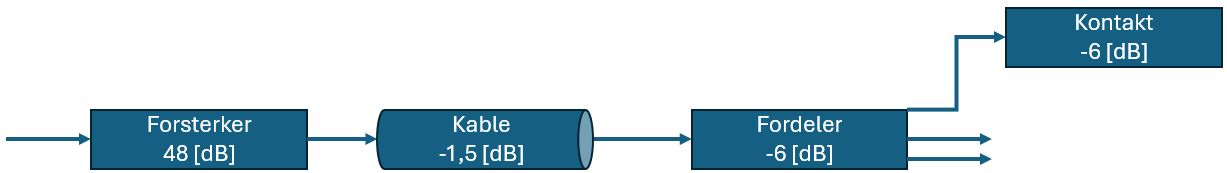
\includegraphics[width=0.9\textwidth]{forsterkning/figurer/forsterkning4.png}
	\caption{Forsterkning i et system}
	\label{fig:forsterk5}
\end{figure}

\end{question}

\vspace{0.5cm} % Add space after the solution

	\begin{solution}[name=Løsningsforslag oppgave]
		\begin{enumerate}[label=\roman*)]
		\item \[L_{F_{tot}}=L_{F_{forsterker}}+L_{F_{kabel}}+L_{F_{kontakt}} = 48+(-1,5)+(-6)+(-3) = 37.5[dB]\]
		\item \[L_{FU}=20 \cdot \log \frac{U_{ut}}{U_{inn}} \rightarrow \frac{L_{FU}}{20}= \log \frac{U_{ut}}{U_{inn}}\]

Tar invers av $\log$.
\[10^{\frac{37,5}{20}}=10^{\log \frac{U_{ut}}{U_{inn}}} \rightarrow 75=\frac{2 \cdot 10^{-3}}{U_{inn}} \rightarrow U_{inn-min}=\frac{2 \cdot 10^{-3}}{75}=26,7[ \mu V]\]

	\end{enumerate}

\end{solution}

\begin{question}[name=Oppgave, topic=forsterkning]
En forsterker for et antennesignal har oppgitt en spenningsforsterkning på $34[dB]$. Finn forsterkningen.

\end{question}

\vspace{0.5cm} % Add space after the solution

\begin{solution}[name=Løsningsforslag oppgave]
\[L_{FU}=20 \cdot \log F \rightarrow 10^{\frac{34}{20}}= 10 \log F \rightarrow F=50,1 \]

\end{solution}

\begin{question}[name=Oppgave, topic=forsterkning]
En koblingsboks har oppgitt en demping av signalet på $3[dB]$. I tillegg er det en demping av signalet i kabelen frem til koblingsboksen på $1[dB]$. Signalet inn i kabelen er $100[\mu V]$ Hva er signalstyrken i koblingsboksen?

\end{question}

\vspace{0.5cm} % Add space after the solution

\begin{solution}[name=Løsningsforslag oppgave]
\[L_{FU-tot}=(-3)+(-1)=-4[dB]\]

\[L_{FU} = 20 \cdot \log \frac{U_{inn}}{U_{ut}} \rightarrow \frac{L_{FU}}{20}= \log \frac{U_{ut}}{U_{inn}}\]

Tar invers av $\log$.
\[10^{\frac{-4}{20}}=10^{\log \frac {U_{ut}}{U_{inn}}} \rightarrow 0,63 = \frac{U_{ut}}{110 \cdot 10^{-6}} \rightarrow U_{ut}=0,63 \cdot 110 \cdot 10^{-6}=69,4[\mu V]\]


\end{solution}



\vspace{0.5cm} % Add space after the solution